\documentclass[12pt]{article}
\usepackage[utf8]{inputenc}
\usepackage{amsmath}
\usepackage{amssymb}
\usepackage{graphicx}

\graphicspath{ {./plots/} }

\newcommand{\rectres}[1]{
\begin{center}
\begin{tabular}{ |c| }
\hline\\
#1\\
\\
\hline
\end{tabular}
\end{center}
}

\newcommand{\qed}{\hfill$\blacksquare$}

\title{Introduction to Numerical Optimization\\Assignment 3}
%\author{Yair Nahum 034462796\\and\\blabla 11111111 }
\author{}

\begin{document}

\maketitle

%\tableofcontents{}

\section{Quasi-Newton Methods}

\subsection{BFGS Method Implementation}
Implementation in code
\subsection{Find  the  Minimum  of  the  Rosenbrock  Function}
Implementation in code\\
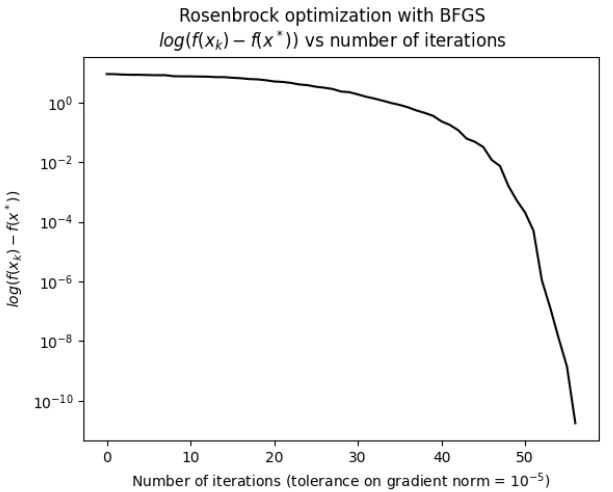
\includegraphics{rosenbrock_BFGS_plot.JPG}\\
The plot seems similar to the newton method rosenbrock convergence and is much better than simple gradient decent rate of convergence. 
\subsection{Neural Networks}
\stepcounter{subsubsection}
\stepcounter{subsubsection}
\stepcounter{subsubsection}
\subsubsection{Explicit Expression of the Neural Network Model}
\begin{itemize}
    \item Hidden layer 1:\\
$$x^1\in \mathbb{R}^{2}, W^1 \in \mathbb{R}^{2\times 4}, b^1\in \mathbb{R}^{4} $$
    \item Hidden layer 2:\\
$$x^2\in \mathbb{R}^{4}, W^2 \in \mathbb{R}^{4\times 3},  b^2\in \mathbb{R}^{3} $$
    \item Output layer:\\
$$x^3\in \mathbb{R}^{3}, W^3 \in \mathbb{R}^{3\times 1},  b^3\in \mathbb{R} $$
\end{itemize}
Now we calculate the layers' outputs:\\
$$x^1 = x$$
$$x^2 = \phi( W^{1^T} x^1 + b^1 )$$
$$x^3 = \phi( W^{2^T} \phi( W^{1^T} x^1 + b^1 ) + b^2)$$
$$F\left(x \vert \mathcal{W}\right) = \phi( W^{3^T} \phi( W^{2^T} \phi( W^{1^T} x^1 + b^1 ) + b^2) + b^3)$$
\stepcounter{subsubsection}
\stepcounter{subsubsection}
\subsubsection{Evaluating  the  Loss  Function’s  Derivative  with  Respect  to  Network’s Output of Single Training Example}
$$\frac{\partial L}{\partial F\left(x^i, \mathcal{W} \right)} = \frac{\partial }{\partial F\left(x^i, \mathcal{W} \right)}\{ \sum_{i=1}^{n} (F(x^i , \mathcal{W}) - y^i )^2\} = 2 (F(x^i , \mathcal{W}) - y^i)$$
\stepcounter{subsubsection}
\stepcounter{subsubsection}
\stepcounter{subsubsection}
\stepcounter{subsubsection}
\stepcounter{subsubsection}
\stepcounter{subsubsection}
\subsubsection{ Combining it All Together}
$\epsilon=0.1$:\\
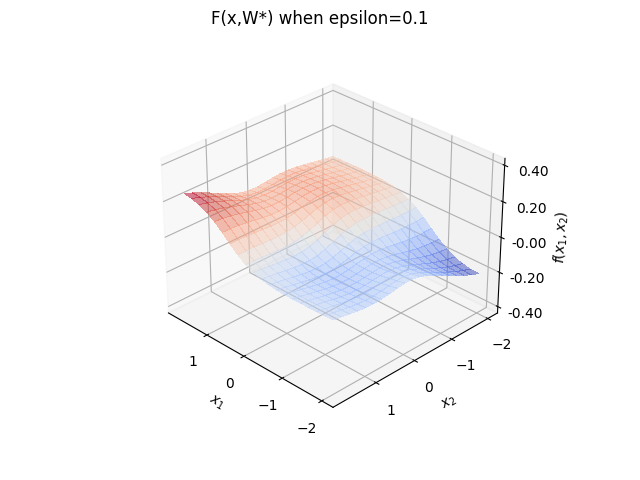
\includegraphics{model_approx_epsilon_0.png}\\
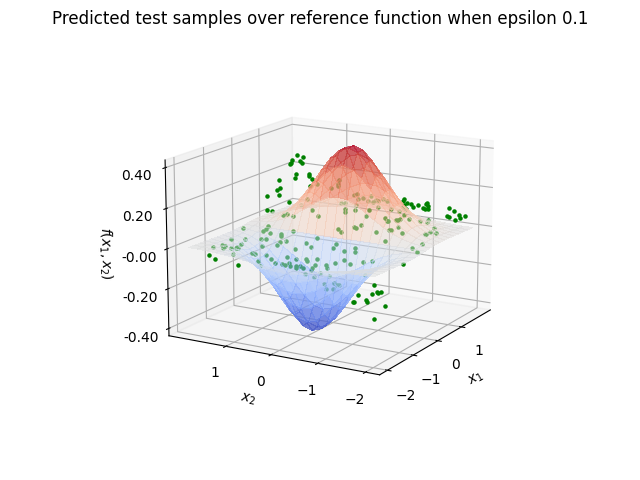
\includegraphics{model_test_over_ref_func_0.png}\\
As seen on plots, with $\epsilon=0.1$ the model approximation is still far and biased from the true function as we didn't train it enough to the needed accuracy (small enough loss or gradient norm).\\
\newpage
$\epsilon=0.01$:\\
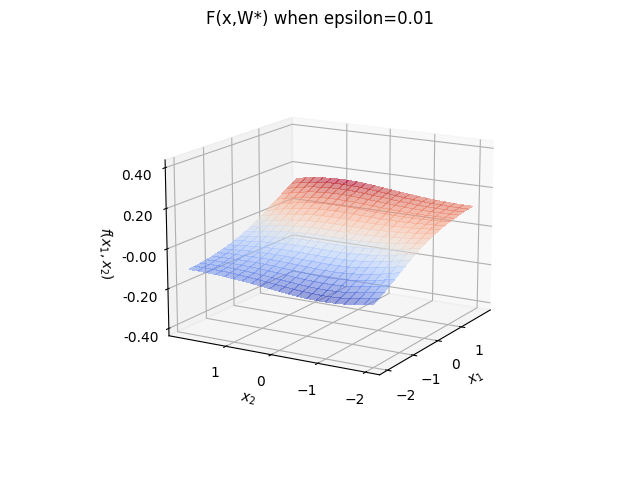
\includegraphics{model_approx_epsilon_1.png}\\
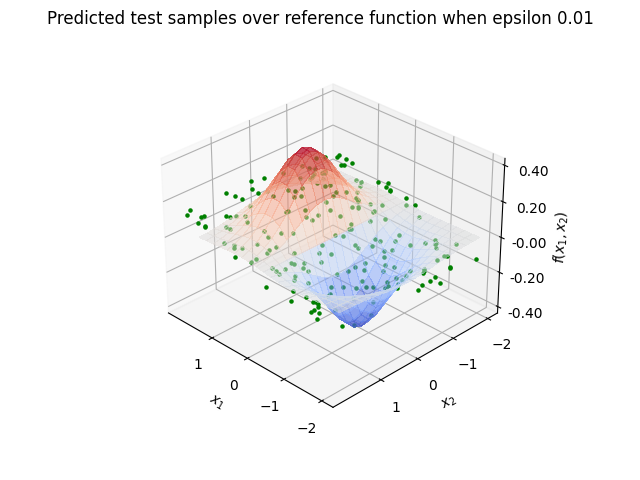
\includegraphics{model_test_over_ref_func_1.png}\\
With $\epsilon=0.01$, we get better approximation compared to the previous one, but still there is a lot of room for improvement as the bias is still big.
\newpage
$\epsilon=0.001$:\\
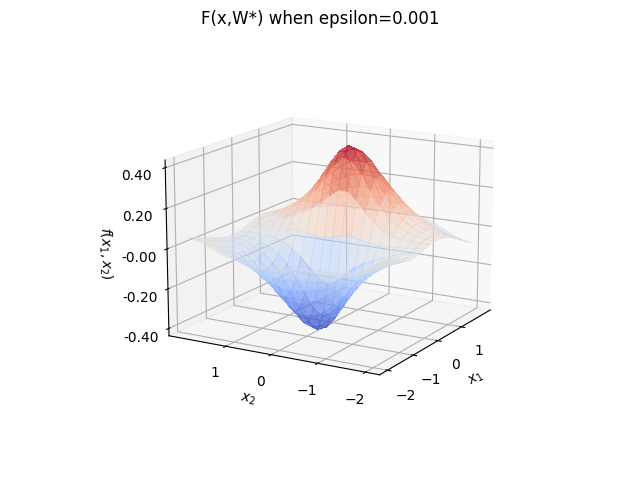
\includegraphics{model_approx_epsilon_2.png}\\
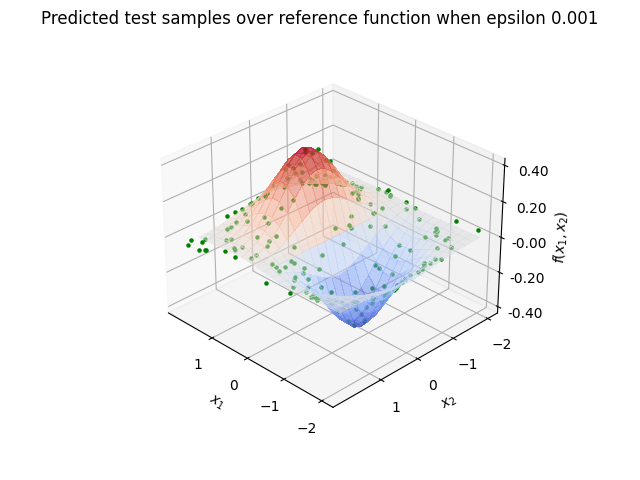
\includegraphics{model_test_over_ref_func_2.png}\\
With $\epsilon=0.001$, we are very close to the true function but still there are mismatches and gaps at the corners as these locations suffer from less data to train on.\\ Training more (with even the same data but with more epochs) gives even better results as we will see next with even smaller $\epsilon$
\newpage
$\epsilon=0.0001$:\\
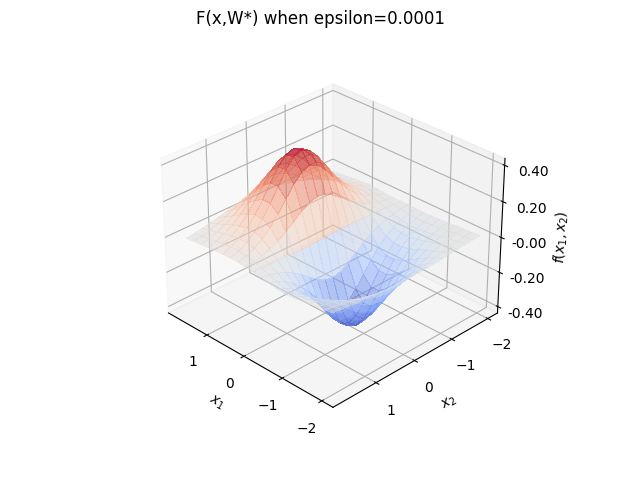
\includegraphics{model_approx_epsilon_3.png}\\
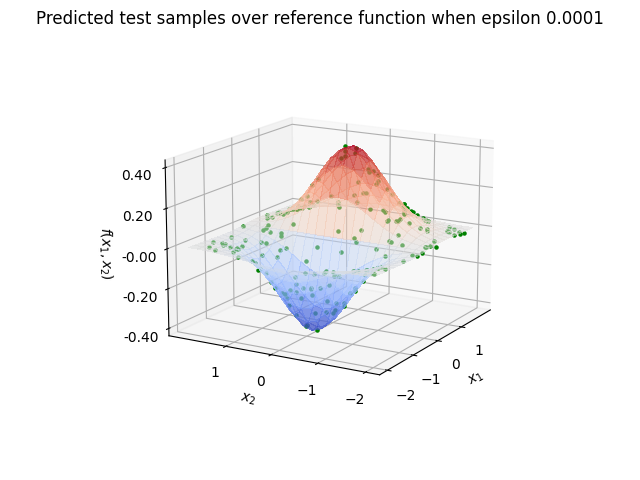
\includegraphics{model_test_over_ref_func_3.png}\\
With $\epsilon=0.0001$, we get smaller less (better minimum point from all others) and due to longer training we get very accurate approximation of the true function.\\
The danger with training on small amount of data is over fitting to the training data, but we can see we didn't get there yet. From plots and final loss it seems to predict almost perfectly the true function.

\end{document}

